\documentclass[8pt, xcolor={svgnames}, hyperref={colorlinks,linkcolor=black, citecolor=amethyst, urlcolor=amethyst}]{beamer}


\usepackage[labelfont={color=amethyst,bf}]{caption}
\usetheme[progressbar=frametitle]{metropolis}
\usepackage{appendixnumberbeamer}
\usepackage{url}
\usepackage{booktabs}
\usepackage{braket}
\usepackage[scale=2]{ccicons}
\usepackage{amsfonts} 
\usepackage{amssymb}
\usepackage[english]{babel}
\colorlet{col1}{teal}
\colorlet{col2}{yellow}
\colorlet{col3}{green}
\usepackage{fontawesome}
\usepackage{multicol}
\usepackage{bm}
\usepackage{algorithm}
\usepackage{algpseudocode}
\usepackage{enumitem}

\usepackage[]{pseudo}


\usepackage{tikz}
\usetikzlibrary{positioning,arrows,calc,math,angles,quotes}
\usepackage{blochsphere}

\usetikzlibrary{arrows,automata}
\usetikzlibrary{positioning}
\usetikzlibrary{arrows.meta,
                bending,
                intersections,
                quotes,
                shapes.geometric}

\tikzset{
    state/.style={
           rectangle,
           rounded corners,
           draw=black, very thick,
           minimum height=1em,
           inner sep=2pt,
           text centered,
           },
}


\definecolor{myv}{rgb}{0.36, 0.22, 0.33}
\definecolor{gio}{rgb}{0.45, 0.31, 0.59}
\definecolor{light}{rgb}{0.8, 0.8, 1}
\definecolor{warmblack}{rgb}{0.0, 0.26, 0.26}
\definecolor{brown(web)}{rgb}{0.65, 0.16, 0.16}
\definecolor{cadmiumgreen}{rgb}{0.0, 0.42, 0.24}
\definecolor{darkmidnightblue}{rgb}{0.0, 0.2, 0.4}
\definecolor{brightube}{rgb}{0.82, 0.62, 0.91}

\definecolor{codegreen}{rgb}{0,0.6,0}
\definecolor{codegray}{rgb}{0.5,0.5,0.5}
\definecolor{codepurple}{rgb}{0.58,0,0.82}
\definecolor{backcolour}{rgb}{0.95,0.95,0.92}
\definecolor{amethyst}{rgb}{0.6, 0.4, 0.8}

\definecolor{light-gray}{gray}{0.95}
\newcommand{\code}[1]{\colorbox{light-gray}{\texttt{#1}}}

\usepackage{listings}
\lstdefinestyle{mystyle}{
    backgroundcolor=\color{backcolour},   
    commentstyle=\color{codegreen},
    keywordstyle=\color{codepurple},
    numberstyle=\tiny\color{codepurple},
    stringstyle=\color{magenta},
    basicstyle=\scriptsize,
    breakatwhitespace=false,         
    breaklines=true,                 
    captionpos=b,                    
    keepspaces=true,                 
    numbers=left,                    
    numbersep=5pt,                  
    showspaces=false,                
    showstringspaces=false,
    showtabs=false,                  
    tabsize=2
}

\lstset{style=mystyle}
\usepackage[most]{tcolorbox}
\usepackage{xcolor}

%\usepackage[citecolor = green, linkcolor = blue, bookmarks=true, urlcolor=blue,
%colorlinks=true, pagebackref=true]{hyperref}



%\usepackage{xspace}

\title{QTI-TH Forum - Hands on Qibo}
\date{Jen. 12, 2023}
\author[Matteo Robbiati]{Matteo Robbiati}
\titlegraphic{
\begin{tikzpicture}[overlay, remember picture]
\node[at=(current page.south east), anchor=south east] {%

\includegraphics[width=.15\textwidth]{figures/unimi.png} \includegraphics[width=.2\textwidth]{figures/infn_logo.png} \includegraphics[width=.25\textwidth]{figures/CERN-Logo.png}  
};
\end{tikzpicture}
}



\begin{document}


\maketitle

\begin{frame}{How was qibo born?}
    \begin{figure}  
    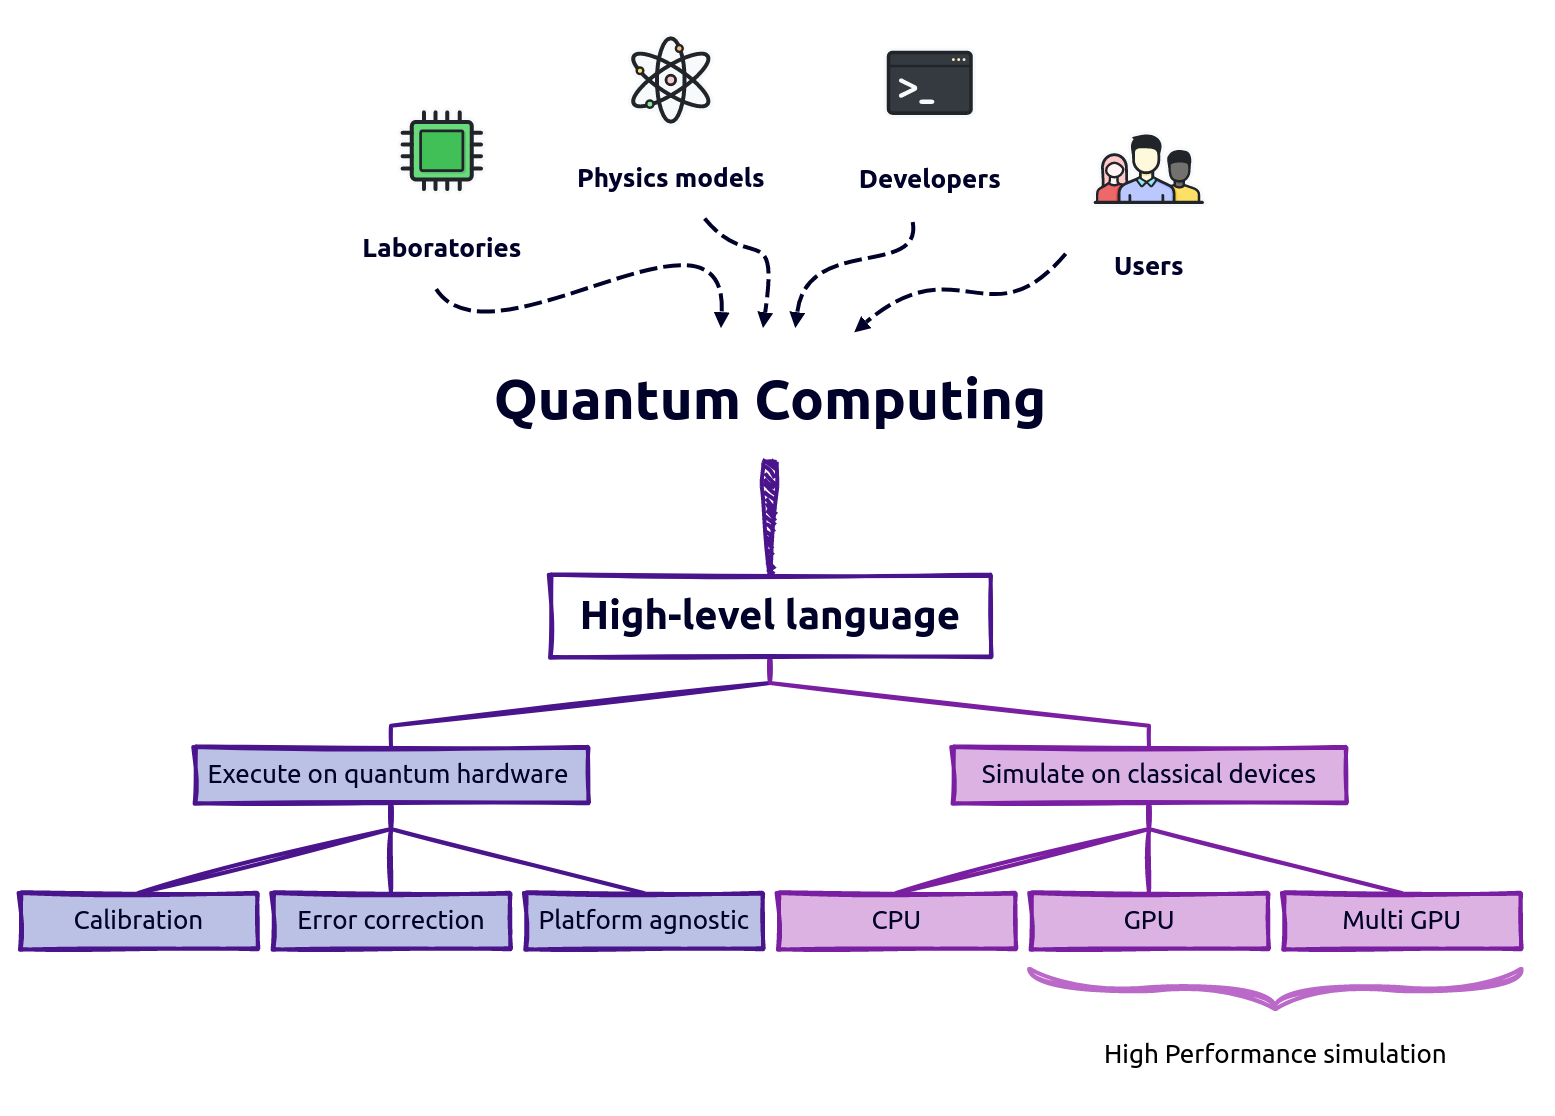
\includegraphics[width=1\textwidth]{figures/Quantum_Computing.png}
    \end{figure}
    \vspace{-0.5cm}
\end{frame}

\section{A snapshot of quantum computing}

\begin{frame}{What is a qubit?}
\large
\faArrowCircleRight\,\, In a quantum computer, bits are replaced by \textbf{qubits},
\pause

\faArrowCircleRight\,\, which, in general, live in a superposition of 
the two \textbf{fundamental states} $\ket{0}$ and $\ket{1}$:
\begin{equation*}
    \ket{\psi} = \alpha \ket{0} + \beta \ket{1}: \,\,
    \begin{pmatrix} 
    \alpha \\ 
    \beta 
    \end{pmatrix}, \qquad \text{with} \qquad     
    \ket{0}:
    \begin{pmatrix} 
    1 \\ 
    0  
    \end{pmatrix}, \qquad \ket{1}:
    \begin{pmatrix} 
    0 \\ 
    1 
    \end{pmatrix}, 
\end{equation*}

and where $\alpha$, $\beta$ $\in \mathbb{C}$, and \textbf{the state is normalized}, i.e. $
    \vert \alpha \vert^2 + \vert \beta \vert^2 = 1.
$   
\pause
\vspace{0.8cm}
\begin{tcolorbox}[colback=amethyst!30, title=Storage advantage]
  The amount of information stored in a quantum device increase \textbf{exponentially}
  with the number of qubits. \\
  
  Example: \textit{a $1024$ pixels img ($32 \times 32$) can be completely represented 
  by a 10-qubits system, whose state vector is $2^{10}=1024$ long!}
\end{tcolorbox}
\end{frame}


\begin{frame}{Gates}
\large
    \faArrowCircleRight\,\, We can act on qubits with \textbf{unitary operators} 
    represented as \textbf{gates}.
    Some of the most important gates are:
    \begin{itemize}
        \item<1->[\faCaretRight] the \textbf{Hadamard} gate
    \begin{equation*}
        H = \frac{1}{\sqrt{2}} \begin{pmatrix} 
        1 & 1 \\ 
        1 & -1
        \end{pmatrix},
    \end{equation*}
    that can be used for building superposition: $H \ket{0} = \frac{1}{\sqrt{2}} (\ket{0} + \ket{1})$.

    \item<2->[\faCaretRight] the \textbf{rotational} gates \color{black}
    \begin{equation*}
        R_i(\theta) = e^{-i \frac{\theta}{2} \sigma_i},
    \end{equation*} in which the Pauli operators appear.

    \item<3->[\faCaretRight] the \textbf{controlled} gates (e.g. c-NOT\only<1,2>{\footnote{\phantom{It 
    acts with a NOT gate on the target qubit only if the control qubit is in the 
    state $\ket{1}$.}}}\only<3->{\footnote{It 
    acts with a NOT gate on the target qubit only if the control qubit is in the 
    state $\ket{1}$.}}), which are used to build entanglement;

    \item<4->[\faCaretRight] the \textbf{measurement gate}, which is the only 
    non-reversible operation we can perform on a quantum system.

 \end{itemize}
    
\end{frame}

\subsection{Bloch sphere representation}

\begin{frame}[fragile]{Bloch sphere visualization}
\large
\faArrowCircleRight\,\, A quantum pure state can be nicely represented using the Bloch 
sphere's notation:
\begin{equation*}
    \alpha = \cos{\frac{\theta}{2}}, \qquad \beta = e^{i\phi}\sin{\frac{\theta}{2}}.
\end{equation*}
\vspace{0.3cm}
\begin{multicols}{2}
\def\rotationSphere{-110}
\def\radiusSphere{2cm}
\def\psiLat{45}
\def\psiLon{45}
\begin{blochsphere}[radius=\radiusSphere,opacity=0,rotation=\rotationSphere]
  % \drawBallGrid[style={opacity=.3}]{30}{45}
  % Draw the sphere...
  \drawLongitudeCircle[]{\rotationSphere}

  \drawLatitudeCircle[style={dashed}]{0}
  % Define the different points on the bloch sphere
  \labelLatLon{ket0}{90}{0};
  \labelLatLon{ket1}{-90}{0};
  \labelLatLon{ketminus}{0}{180};
  \labelLatLon{ketplus}{00}{0};
  \labelLatLon{ketpluspi2}{0}{-90};  % Longitude seems to be defined in the "wrong" direction, hence the minus
  \labelLatLon{ketplus3pi2}{0}{-270};
  \labelLatLon{psi}{\psiLat}{-\psiLon};
  % Draw and label the axis
  \draw[-latex] (0,0) -- (ket0) node[above,inner sep=.5mm] at (ket0) {\footnotesize $z$};
  \draw[-latex] (0,0) -- (ketplus) node[below,inner sep=.5mm] at (ketplus) {\footnotesize$x$};
  \draw[-latex] (0,0) -- (ketpluspi2) node[below,inner sep=.5mm] at (ketpluspi2) {\footnotesize $y$};
  % Draw |psi>
  \draw[-latex] (0,0) -- (psi) node[above]{\footnotesize $\ket{\psi}$};

  % Draw the angles
  \coordinate (origin) at (0,0);
  {
    % Will draw the angle/projection one the equatorial plane
    \setDrawingPlane{0}{0}
    % Draw the projection: cos is used to compute the length of the projection
    \draw[current plane,dashed] (0,0) -- (-90+\psiLon:{cos(\psiLat)*\radiusSphere}) coordinate (psiProjectedEquat) -- (psi);
    % Draw the angle
    \pic[current plane, draw,fill=purple!50,fill opacity=.5, text opacity=1,"\footnotesize $\phi$", angle eccentricity=2.2]{angle=ketplus--origin--psiProjectedEquat};
  }
  { \setLongitudinalDrawingPlane{\psiLon}
    % Draw the angle
    \pic[current plane, draw,fill=purple!50,fill opacity=.5, text opacity=1,"\footnotesize $\theta$", angle eccentricity=1.5]{angle=psi--origin--ket0};
  }
\end{blochsphere}
\end{multicols}
\end{frame}


\begin{frame}[fragile]{Bloch sphere visualization - RX}
\large
\faArrowCircleRight\,\, A quantum state can be nicely represented using the Bloch sphere's notation:
\begin{equation*}
    \alpha = \cos{\frac{\theta}{2}}, \qquad \beta = e^{i\phi}\sin{\frac{\theta}{2}}.
\end{equation*}
\vspace{0.3cm}
\begin{multicols}{2}
\def\rotationSphere{-110}
\def\radiusSphere{2cm}
\def\psiLat{45}
\def\psiLon{45}
\begin{blochsphere}[radius=\radiusSphere,opacity=0,rotation=\rotationSphere]
  % \drawBallGrid[style={opacity=.3}]{30}{45}
  % Draw the sphere...
  \drawLongitudeCircle[]{\rotationSphere}
  \drawRotationRight[scale=1.3,style={amethyst}]{90}{0}{0}{5}

  \drawLatitudeCircle[style={dashed}]{0}
  % Define the different points on the bloch sphere
  \labelLatLon{ket0}{90}{0};
  \labelLatLon{ket1}{-90}{0};
  \labelLatLon{ketminus}{0}{180};
  \labelLatLon{ketplus}{00}{0};
  \labelLatLon{ketpluspi2}{0}{-90};  % Longitude seems to be defined in the "wrong" direction, hence the minus
  \labelLatLon{ketplus3pi2}{0}{-270};
  \labelLatLon{psi}{\psiLat}{-\psiLon};
  % Draw and label the axis
  \draw[-latex] (0,0) -- (ket0) node[above,inner sep=.5mm] at (ket0) {\footnotesize $z$};
  \draw[-latex] (0,0) -- (ketplus) node[below,inner sep=.5mm] at (ketplus) {\footnotesize$x$};
  \draw[-latex] (0,0) -- (ketpluspi2) node[below,inner sep=.5mm] at (ketpluspi2) {\footnotesize $y$};
  % Draw |psi>
  \draw[-latex] (0,0) -- (psi) node[above]{\footnotesize $\ket{\psi}$};

  % Draw the angles
  \coordinate (origin) at (0,0);
  {
    % Will draw the angle/projection one the equatorial plane
    \setDrawingPlane{0}{0}
    % Draw the projection: cos is used to compute the length of the projection
    \draw[current plane,dashed] (0,0) -- (-90+\psiLon:{cos(\psiLat)*\radiusSphere}) coordinate (psiProjectedEquat) -- (psi);
    % Draw the angle
    \pic[current plane, draw,fill=purple!50,fill opacity=.5, text opacity=1,"\footnotesize $\phi$", angle eccentricity=2.2]{angle=ketplus--origin--psiProjectedEquat};
  }
  { \setLongitudinalDrawingPlane{\psiLon}
    % Draw the angle
    \pic[current plane, draw,fill=purple!50,fill opacity=.5, text opacity=1,"\footnotesize $\theta$", angle eccentricity=1.5]{angle=psi--origin--ket0};
  }
\end{blochsphere}

\begin{itemize}
    \item[\faTerminal] \textcolor{amethyst}{Rotation around the $x$ axis;} 
\end{itemize}
\end{multicols}
\end{frame}

\begin{frame}[fragile]{Bloch sphere visualization - RY}
\large
\faArrowCircleRight\,\, A quantum state can be nicely represented using the Bloch sphere's notation:
\begin{equation*}
    \alpha = \cos{\frac{\theta}{2}}, \qquad \beta = e^{i\phi}\sin{\frac{\theta}{2}}.
\end{equation*}
\vspace{0.3cm}
\begin{multicols}{2}
\def\rotationSphere{-110}
\def\radiusSphere{2cm}
\def\psiLat{45}
\def\psiLon{45}
\begin{blochsphere}[radius=\radiusSphere,opacity=0,rotation=\rotationSphere]
  % \drawBallGrid[style={opacity=.3}]{30}{45}
  % Draw the sphere...
  \drawLongitudeCircle[]{\rotationSphere}
  \drawRotationRight[scale=1.3,style={amethyst}]{90}{90}{0}{5}

  \drawLatitudeCircle[style={dashed}]{0}
  % Define the different points on the bloch sphere
  \labelLatLon{ket0}{90}{0};
  \labelLatLon{ket1}{-90}{0};
  \labelLatLon{ketminus}{0}{180};
  \labelLatLon{ketplus}{00}{0};
  \labelLatLon{ketpluspi2}{0}{-90};  % Longitude seems to be defined in the "wrong" direction, hence the minus
  \labelLatLon{ketplus3pi2}{0}{-270};
  \labelLatLon{psi}{\psiLat}{-\psiLon};
  % Draw and label the axis
  \draw[-latex] (0,0) -- (ket0) node[above,inner sep=.5mm] at (ket0) {\footnotesize $z$};
  \draw[-latex] (0,0) -- (ketplus) node[below,inner sep=.5mm] at (ketplus) {\footnotesize$x$};
  \draw[-latex] (0,0) -- (ketpluspi2) node[below,inner sep=.5mm] at (ketpluspi2) {\footnotesize $y$};
  % Draw |psi>
  \draw[-latex] (0,0) -- (psi) node[above]{\footnotesize $\ket{\psi}$};

  % Draw the angles
  \coordinate (origin) at (0,0);
  {
    % Will draw the angle/projection one the equatorial plane
    \setDrawingPlane{0}{0}
    % Draw the projection: cos is used to compute the length of the projection
    \draw[current plane,dashed] (0,0) -- (-90+\psiLon:{cos(\psiLat)*\radiusSphere}) coordinate (psiProjectedEquat) -- (psi);
    % Draw the angle
    \pic[current plane, draw,fill=purple!50,fill opacity=.5, text opacity=1,"\footnotesize $\phi$", angle eccentricity=2.2]{angle=ketplus--origin--psiProjectedEquat};
  }
  { \setLongitudinalDrawingPlane{\psiLon}
    % Draw the angle
    \pic[current plane, draw,fill=purple!50,fill opacity=.5, text opacity=1,"\footnotesize $\theta$", angle eccentricity=1.5]{angle=psi--origin--ket0};
  }
\end{blochsphere}

\begin{itemize}

    \item[\faTerminal] Rotation around the $x$ axis;
    \item[\faTerminal] \textcolor{amethyst}{Rotation around the $y$ axis;} 
\end{itemize}
\end{multicols}
\end{frame}

\begin{frame}[fragile]{Bloch sphere visualization - RZ}
\large
\faArrowCircleRight\,\, A quantum state can be nicely represented using the Bloch sphere's notation:
\begin{equation*}
    \alpha = \cos{\frac{\theta}{2}}, \qquad \beta = e^{i\phi}\sin{\frac{\theta}{2}}.
\end{equation*}
\vspace{0.3cm}
\begin{multicols}{2}
\def\rotationSphere{-110}
\def\radiusSphere{2cm}
\def\psiLat{45}
\def\psiLon{45}
\begin{blochsphere}[radius=\radiusSphere,opacity=0,rotation=\rotationSphere]
  % \drawBallGrid[style={opacity=.3}]{30}{45}
  % Draw the sphere...
  \drawLongitudeCircle[]{\rotationSphere}
  \drawRotationRight[scale=1.3,style={amethyst}]{0}{0}{0}{5}

  \drawLatitudeCircle[style={dashed}]{0}
  % Define the different points on the bloch sphere
  \labelLatLon{ket0}{90}{0};
  \labelLatLon{ket1}{-90}{0};
  \labelLatLon{ketminus}{0}{180};
  \labelLatLon{ketplus}{00}{0};
  \labelLatLon{ketpluspi2}{0}{-90};  % Longitude seems to be defined in the "wrong" direction, hence the minus
  \labelLatLon{ketplus3pi2}{0}{-270};
  \labelLatLon{psi}{\psiLat}{-\psiLon};
  % Draw and label the axis
  \draw[-latex] (0,0) -- (ket0) node[above,inner sep=.5mm] at (ket0) {\footnotesize $z$};
  \draw[-latex] (0,0) -- (ketplus) node[below,inner sep=.5mm] at (ketplus) {\footnotesize$x$};
  \draw[-latex] (0,0) -- (ketpluspi2) node[below,inner sep=.5mm] at (ketpluspi2) {\footnotesize $y$};
  % Draw |psi>
  \draw[-latex] (0,0) -- (psi) node[above]{\footnotesize $\ket{\psi}$};

  % Draw the angles
  \coordinate (origin) at (0,0);
  {
    % Will draw the angle/projection one the equatorial plane
    \setDrawingPlane{0}{0}
    % Draw the projection: cos is used to compute the length of the projection
    \draw[current plane,dashed] (0,0) -- (-90+\psiLon:{cos(\psiLat)*\radiusSphere}) coordinate (psiProjectedEquat) -- (psi);
    % Draw the angle
    \pic[current plane, draw,fill=purple!50,fill opacity=.5, text opacity=1,"\footnotesize $\phi$", angle eccentricity=2.2]{angle=ketplus--origin--psiProjectedEquat};
  }
  { \setLongitudinalDrawingPlane{\psiLon}
    % Draw the angle
    \pic[current plane, draw,fill=purple!50,fill opacity=.5, text opacity=1,"\footnotesize $\theta$", angle eccentricity=1.5]{angle=psi--origin--ket0};
  }
\end{blochsphere}

\begin{itemize}

    \item[\faTerminal] Rotation around the $x$ axis;
    \item[\faTerminal] Rotation around the $y$ axis; 
    \item[\faTerminal] \textcolor{amethyst}{Rotation around the $z$ axis.} 
\end{itemize}
\end{multicols}
\end{frame}

\subsection{Why we mention rotations?}

\begin{frame}{Why we mention rotations?}
\large 
    \faArrowCircleRight\,\, Many variational models in quantum computations involve 
    rotations.
    
    \faArrowCircleRight\,\, It is easy to embed an input variable into a model if 
    passed as rotation angle.

    \begin{figure}
    \centering 
    \includegraphics[width=0.9\textwidth]{figures/variational_model.png}
  \caption{Example of how can we use a circuit as variational model.}
  \end{figure}
\end{frame}

\section{From theory to deployment}

\begin{frame}{What can be a qubit for real?}
    \begin{figure}
    \centering 
    \includegraphics[width=\textwidth]{figures/Quantum_tech.png}
  \caption{Common qubit's technologies. Graphic by C. Bickle/Science data by Gabriel Popkin.}
  \end{figure}
\end{frame}

\begin{frame}{Superconducting qubit}
\begin{multicols}{2}
\begin{figure}
    \centering 
    \includegraphics[width=0.4\textwidth]{figures/photon_absorb.png}
\end{figure}
\pause
\begin{figure}
    \centering 
    \includegraphics[width=0.4\textwidth]{figures/LC_circuit.png}
\end{figure}
\end{multicols}  
\begin{multicols}{2}
\pause
\begin{figure}
    \centering 
    \includegraphics[width=0.4\textwidth]{figures/JC_circuit.png}
\end{figure}
\pause
\begin{figure}
    \centering 
    \includegraphics[width=0.4\textwidth]{figures/energy_levels.png}
\end{figure}
\end{multicols}
Images reference: \href{https://pennylane.ai/qml/demos/tutorial_sc_qubits.html}{here}.  
\end{frame}

\begin{frame}{From theory to deployment - the simple NOT gate example}

\large

Let's suppose we want to build a NOT ($X$) gate using a \textbf{superconducting}
qubit. 
\vspace{0.3cm}
\pause 
\begin{itemize}
    \item[\faPencilSquareO] Theoretically, we know that $X$ must \textbf{swap} 
    the two fundamental states when acting on them;
    \pause
    \item[\faTerminal] we want to \textbf{easily code} this on our console for doing:
    \begin{itemize}
        \item[\tiny\faCircle] \textbf{simulation} on our classical computer;
        \item[\tiny\faCircle] \textbf{real quantum computation} if we have access to a lab; 
    \end{itemize}
    \pause
    \item[\faWrench] in the second case, $X$ must be \textbf{implemented} 
    as a sequence of pulses $P$ which can swap the two fundamental states 
    (\textbf{quantum control});
    \pause
    \item[\faSliders] each qubit built in the "foundry" is different: 
    we need to \textbf{fine-tune} $P$ to optimize the interpretation of $X$ 
    (\textbf{quantum calibration}).
\end{itemize}

\pause
\vspace{0.2cm}
\begin{tcolorbox}[colback=amethyst!30, title=Some more info]
  The ground state can be easily obtained by bringing the circuit
  temperature next to $T=0$K\footnote{In the TII lab the cryostats keep quantum chips act
  $T\sim$mK}.
\end{tcolorbox}
\end{frame}

\section{Presenting \texttt{qibo}}

\begin{frame}{From theory to deployment - \texttt{qibo}}
\large
\faArrowCircleRight\,\, \texttt{qibo} is a \textbf{totally open-source} and \textbf{full-stack} 
framework which well-fits with the scientific research context.
    \begin{figure}
    \centering 
    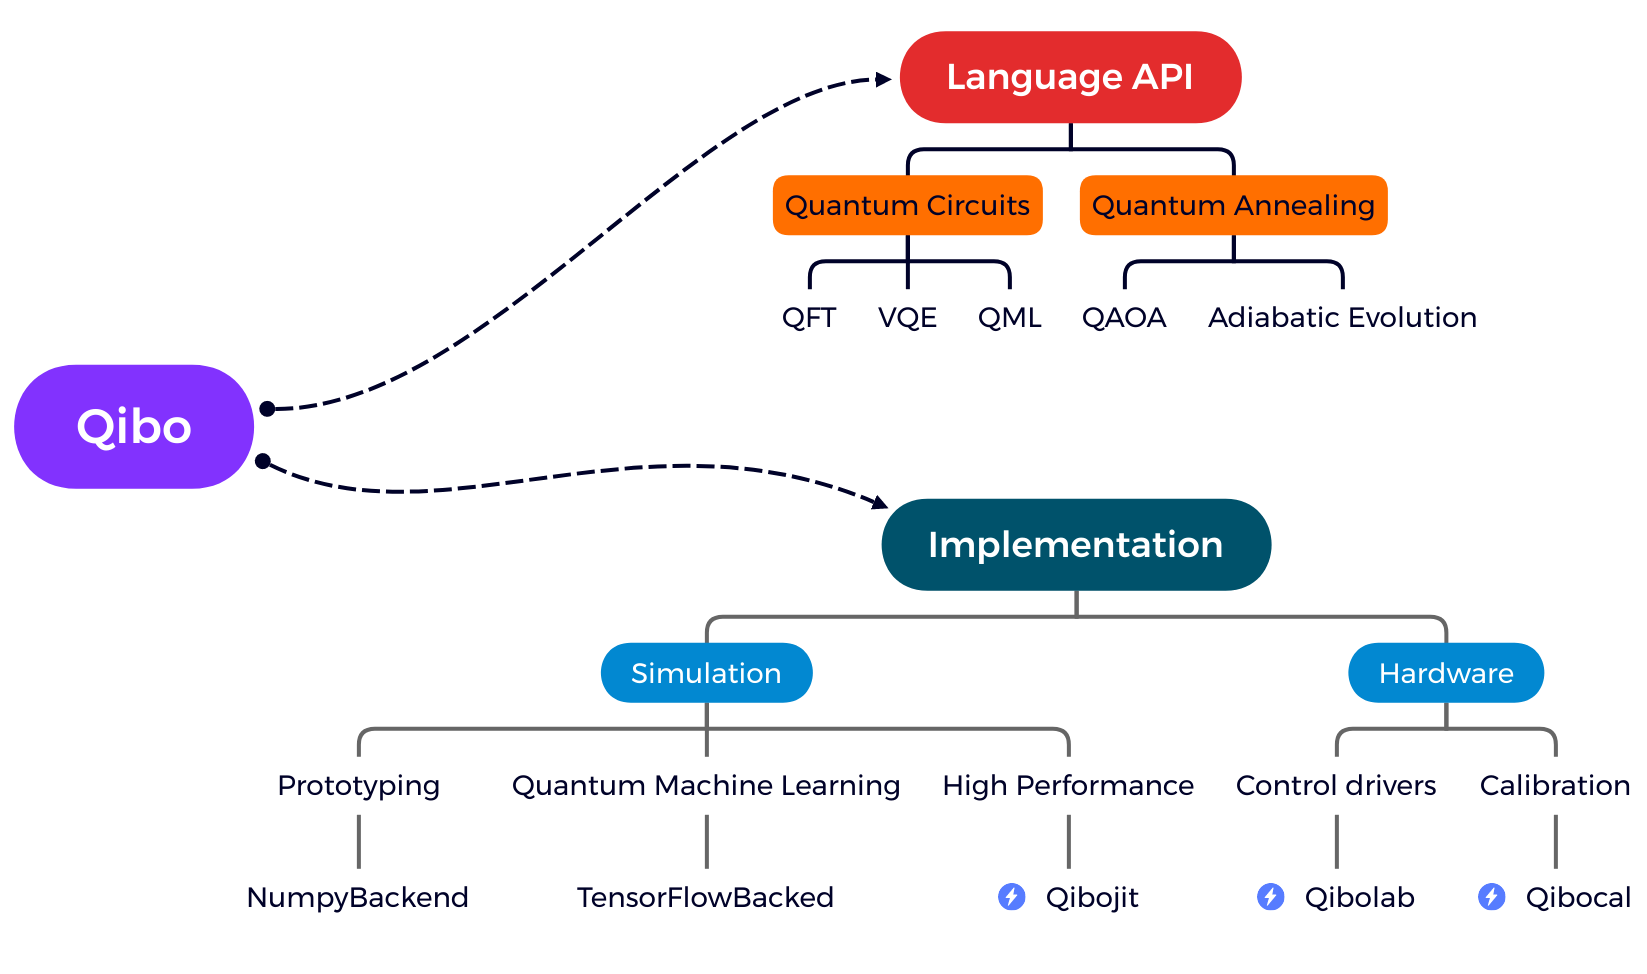
\includegraphics[width=\textwidth]{figures/Qibo.png}
  \end{figure}
  \faBook\,\, \href{https://arxiv.org/abs/2009.01845}{arXiv:2009.01845}
\end{frame}

\begin{frame}{\texttt{qibojit} for simulating a larger number of qubits}
\large 

\faArrowCircleRight\,\, Since we do \textbf{state vector simulation} via linear 
algebra, the goal is to limit the calculation time.

\faArrowCircleRight\,\, \texttt{qibojit} is an efficient simulation backend for 
CPU, GPU and multi-GPU based on just-in-time (JIT) compiled custom operators. 

    \begin{figure}
    \centering 
    \includegraphics[width=0.8\textwidth]{figures/qibojit-qft.png}
  \end{figure}
  
  \faBook\,\, \href{https://arxiv.org/abs/2203.08826}{arXiv:2203.08826}
\end{frame}

\begin{frame}{\texttt{qibojit} vs other libraries}
\large 

\begin{figure}
    \centering 
    \includegraphics[width=1\textwidth]{figures/libraries.png}
\end{figure}

\begin{figure}
    \centering 
    \includegraphics[width=1\textwidth]{figures/lib-2.png}
  \end{figure}
    
\end{frame}

\section{Why use \texttt{qibo} in my lab?}


\begin{frame}{A full-stack framework for self-hosted quantum devices}
\large 
\faArrowCircleRight\,\, Can \texttt{qibo} be used to simulate, control and calibrate
a \textbf{self-hosted} quantum device?

\pause

\faArrowCircleRight\,\, Yes! It is \textbf{hardware-agnostic}, open source and 
available to be used. 

\pause

\faArrowCircleRight\,\, We only need to describe the hardware specifities into a 
\textbf{custom} \texttt{Platform} object in \texttt{qibolab}.  
It will deploy the theoretical laws (gates, i.e., unitary operations) into the 
proper pulses sequence.

\pause

\faArrowCircleRight\,\, Some \textbf{labs} are already using \texttt{qibo}!

\begin{multicols}{4}
\begin{figure}
    \centering 
    \includegraphics[width=0.2\textwidth]{figures/infn.png}
\end{figure}
\begin{figure}
    \centering 
    \includegraphics[width=0.2\textwidth]{figures/tii.png}
\end{figure}
\begin{figure}
    \centering 
    \includegraphics[width=0.2\textwidth]{figures/cqt.png}
\end{figure}
\begin{figure}
    \centering 
    \includegraphics[width=0.18\textwidth]{figures/bsc.jpg}
\end{figure}
\end{multicols}

\faBook\,\, \href{https://arxiv.org/abs/2202.07017}{arXiv:2202.07017}
\end{frame}

\begin{frame}{How to exploit \texttt{qibo} modularity}
  \begin{figure}
    \centering 
    \includegraphics[width=\textwidth]{figures/qibolab_use.png}
  \end{figure}
\end{frame}

\begin{frame}{Let's jump to the console}
\large
\faArrowCircleRight\,\, We leave some references and links thanks to which you can use our codes and read more about the project:

\begin{multicols}{2}
    
\begin{itemize}
\item[\faCode] open-access codes for personal coding or contributing:
    \begin{itemize}[noitemsep]
        \item[\faGithub]  \href{https://github.com/qiboteam/qibo}{the \texttt{qibo} package};
        \item[\faGithub]  \href{https://github.com/qiboteam/qibolab}{the \texttt{qibolab} package};
        \item[\faGithub]  \href{https://github.com/qiboteam/qibocal}{the \texttt{qibocal} package};
    \end{itemize}
 \vspace{1cm}

\item[\faBook] our official \href{https://qibo.science/}{webpage}, with the following documentations:
    \begin{itemize}[noitemsep]
        \item[\faLeanpub]  \href{https://qibo.science/docs/qibo/stable}{the \texttt{qibo} docs};
        \item[\faLeanpub]  \href{https://qibo.science/docs/qibolab/stable}{the \texttt{qibolab} docs};
        \item[\faLeanpub]  \href{https://qibo.science/docs/qibocal/stable}{the \texttt{qibocal} docs};
    \end{itemize}
\end{itemize}
\end{multicols}

\faCloudDownload\,\, the \href{https://colab.research.google.com/drive/1DoLOS3hsOM3cbzquAI73bmp_fTY3car8\#scrollTo=MmNVieFoGbQU}{Colab notebook} we are going to run together.

\end{frame}


\end{document}
